% Search for all the places that say "PUT SOMETHING HERE".

\documentclass[11pt]{article}
\usepackage{cube,amsmath,textcomp,amssymb,geometry,graphicx,enumerate,tabu}

\def\Session{Fall 2018}

% \title{Syllabus}
\author{\Name, SID \SID}
% \pagestyle{headings}
\date{}

\newenvironment{qparts}{\begin{enumerate}[{(}a{)}]}{\end{enumerate}}
\def\endproofmark{$\Box$}
% \newenvironment{proof}{\par{\bf Proof}:}{\endproofmark\smallskip}

\textheight=9in
\textwidth=6.5in
\topmargin=-.75in
\oddsidemargin=0.25in
\evensidemargin=0.25in


\begin{document}
\maketitle
\title{Course Syllabus}
\centerline{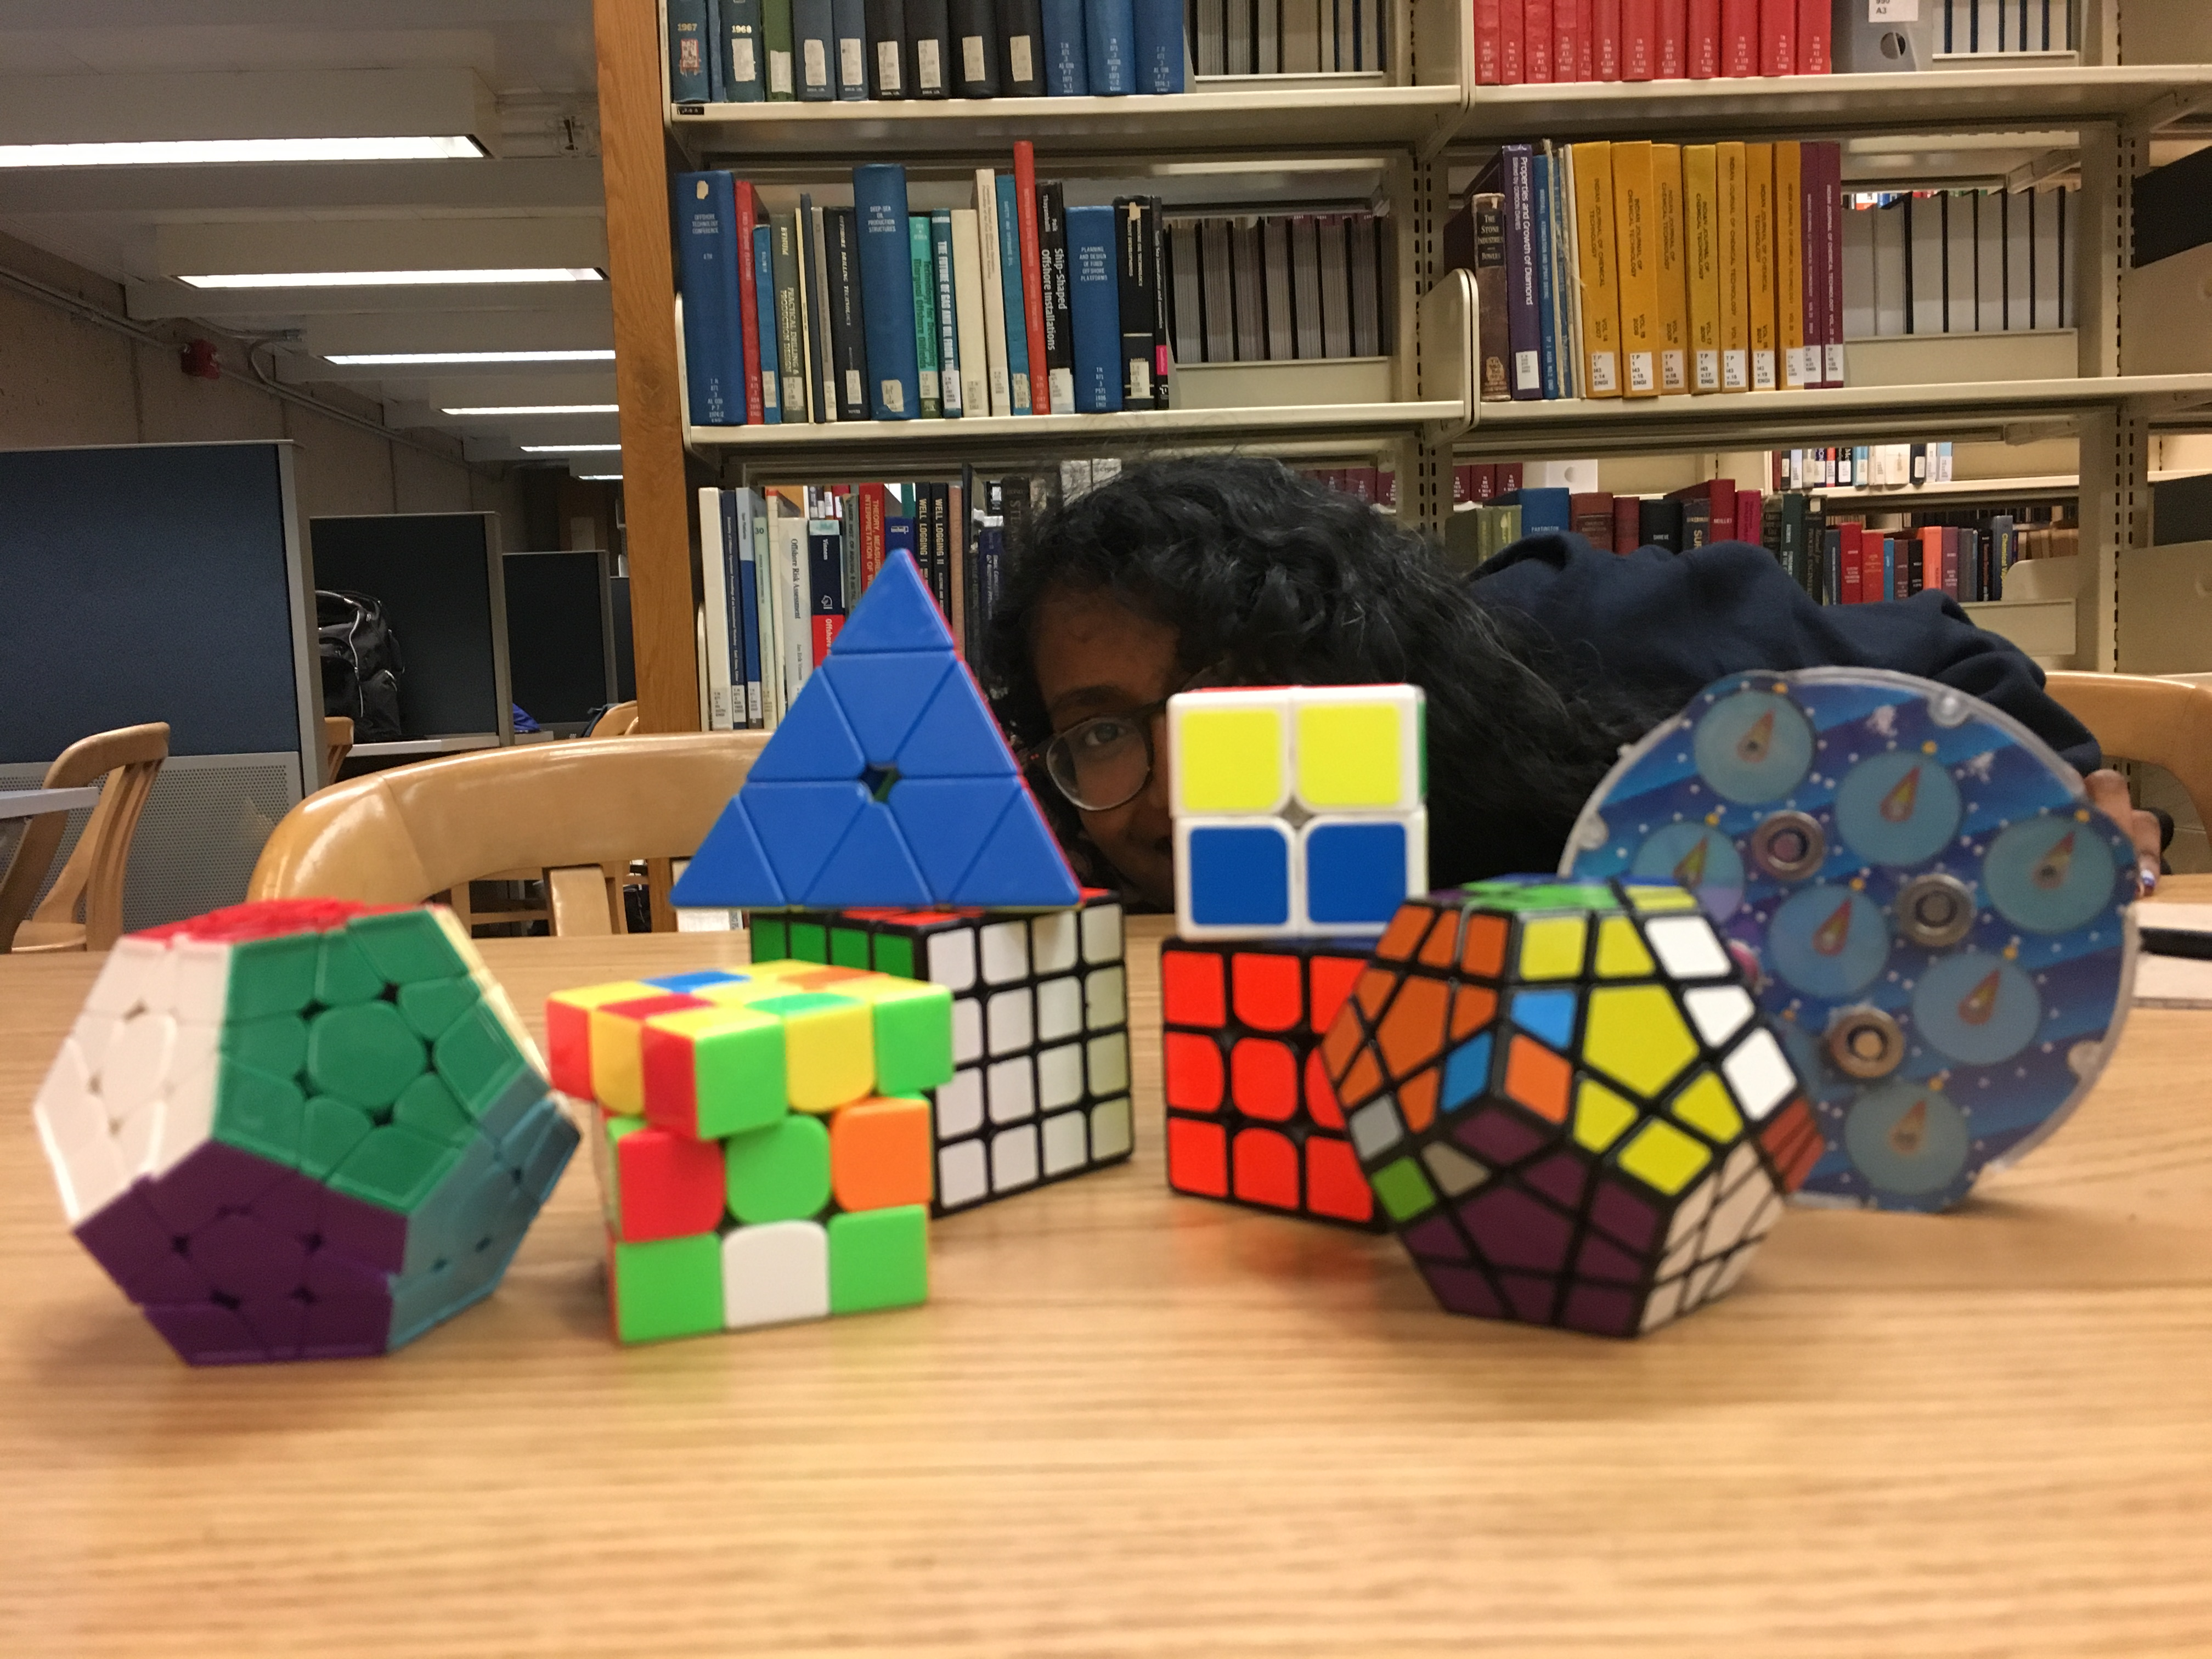
\includegraphics[width=10cm]{5.JPG}}

$\textbf{Semester}$: Spring 2018\\
$\textbf{Room}$: TBD\\
$\textbf{Time}$: Tuesdays 5-7 PM (Beginners 5-6 PM, Advanced 6-7 PM)\\
$\textbf{Starting Date}$: January 30th\\
$\textbf{Facilitators}$: Ryan Jew, Jiazheng Zhao, Abhimanyu Singhal\\
$\textbf{Faculty Sponsor}$: TBD\\
$\textbf{Office Hours}$: After class/By appointment/Instructor Email \\
$\textbf{Grading}$: 1 unit P/NP only

\section*{Objective}
In this DeCal, you will learn how to solve the Rubik’s Cube (Beginner section) or how to solve it much more quickly and efficiently (Advanced section). You will also leave with better problem solving abilities, improved understanding on the history and mathematics of the Rubik’s Cube, improved hand-eye coordination, increased finger dexterity, and a cool party trick.


\section*{Format}
The format of this class will be a combination of lecture and group instruction, with a heavy emphasis on the latter. At the beginning of each class, we will give a brief overview of the lesson and then break into groups for the remainder of the hour. In these groups, you will practice the lessons taught during lecture with personal guidance from your group instructor (you will stay with the same instructor for the entire semester).

\section*{Content}
In the Beginner section, we will be teaching the Layer-By-Layer method, which involves solving the cube “from the ground up”. In the last few weeks of class, we will be holding instruction on various topics such as solving the cube faster and solving other puzzles. 

If you finish the basic curriculum early on, you will have the opportunity to learn more of these topics from your instructor.

In the Advanced section, we will be teaching the Fridrich method, a more advanced version of the Layer-By-Layer method that many people learn. In addition, since more one-on-one instruction is available in the Advanced section, the class is much more flexible. If you have a particular cube-related topic that you would really like to learn, chances are there is an instructor that can teach it to you while or after you learn the regular curriculum. Just be aware that we expect you to fully learn the Fridrich method that we teach, and utilize it in your solving (during the final and competition). Anything after that is up to you.



\section*{Workload}
\subsection*{Come to class}
This is mandatory, as we will introduce a new topic each week and move pretty quickly through the steps. If you miss a class, you will be behind on material. Attendance will be taken weekly by your instructors — if you must miss a class, please let your instructor know ahead of time (unless it’s an emergency). We will allow 3 absences, either excused or unexcused. If you have 4 absences, we will fail you \textbf{without exception}.

\subsection*{Work outside of class}
Besides coming to class, you will need to practice on your Rubik’s Cube outside of class. This can be as little as 15 minutes per day, but obviously the more the better. Practice hones your skills and helps you identify problem areas that you can then ask your instructor about during class. If you practice consistently, you will easily be able learn the regular curriculum within the first few weeks.  Additionally, you must read articles assigned every other week to further supplement your learning experience.

\subsection*{Do the readings}
In both sections, there will be required biweekly readings consisting of articles and short documents on various aspects of the Rubik’s Cube.  These articles will mainly highlight the mathematics and the historical prevalence of the Rubik’s Cube and its other isomorphic structures.  Students will be required to submit a short reflection on each of the readings.

\subsection*{Pass the final}
For the Beginner section, this means solving the cube once in under 5 minutes. You will have up to 5 attempts, if necessary. If you successfully solve the cube on your first try, you pass the class and do not have to complete your remaining attempts (unless you want to).

For the Advanced section, this means solving the cube in under 1 minute 15 seconds. You must complete all five solves to pass.

Additionally, for both sections, there will be a take-home final consisting of short answer and multiple-choice questions and a creative final writing assignment. This also includes doing the various readings throughout the semester and submitting the reflections.
The take-home final will test students on the semester’s readings and mathematical content.
The writing assignment must include mathematical and historical facts about the Rubik's Cube. This is intentionally open-ended: creativity is encouraged!


\subsection*{Participate in a competition}
(Advanced only, although Beginners are encouraged to go) - Advanced students are expected to register and go to one of the official WCA competitions during the semester (www.worldcubeassociation.org). The Bay Area traditionally has 3-5 competitions per semester, at Berkeley, South Bay, etc. We will let you know the dates of the competitions as they become known to us. If it turns out that you cannot make any of the competitions, please let us know as early as possible, and we will work something out. Typically, competitions are held on-campus for a few hours on either Saturday or Sunday.\\
Note: You must complete all of these requirements to pass this class. Failure to do so will result in a grade of NP (no pass).


\section*{Grading}
In addition to completing all the mandatory requirements for both the Beginner’s and Advanced section, a total cumulative grade of 70\% must be achieved in order to pass the class.  The breakdown is as follows:

\begin{center}
	\begin{tabular}{|| c | c ||}
	\hline
	Solve Cube & 40\% \\
	\hline
	Papers and Assignments* & 30\% \\
	\hline
	Final & 30\% \\
	\hline
	\end{tabular}
\end{center}

*Short readings + quizzes will be assigned throughout the semester. Readings are TBD. 


\section*{Prerequisites and Materials}
For the Beginner section, the only prerequisite is that you have your own Rubik’s Cube to practice on. You will not be allowed to share with any other students. No other experience with the Rubik’s Cube or other puzzles is necessary, as we will teach you how to solve it from scratch.

For the Advanced section, you will also need your own Rubik’s Cube to practice with. You will not be allowed to share with any other students. In addition, you must already know how to solve the cube using any method before the first day of class. We would prefer that you know the layer-by-layer method; if you know another method, let us know so that we can tailor the course to meet your needs. This ensures that you have some experience with the cube and that you have some basic intuition with respect to how the cube works.

We may have Rubik’s Cubes available for purchase, but stock is limited. We generally sell cubes for \$5 at the beginning of the course but students may also choose to buy cubes on their own.

If you are confused on which section you belong in, talk to one of the facilitators during the first class, and we will determine which section you should take.



\section*{Other Policies}
In order for the class to proceed smoothly, it should be free of any distractions: \\
Cell Phones - should be left on silent.\\
Tardiness - you should show up by 10 minutes after the hour (Berkeley time).\\
DSP Accomodations - come talk to us or send the instructors an email

\section*{Enrollment}
Deadline to fill out the application listed on the DeCal website — January 26th
We will select ~120 applicants and send them an email with the CCNs on January 28th
The CCNs will be made available to everyone on the DeCal website on January 30th
First class is on January 30th
The CCNs will be taken off from the DeCal website on February 2nd
Beginner’s finals will be held on the last two weeks of class. Advanced finals will be held on the last week of class. More information will be presented in class.

See the DeCal website for further details.

\newpage

\section*{Schedule}
\begin{center}
	\begin{tabu} to .8\textwidth {|| c | c | c | c ||}
	\hline
	Class Date & Beginner's & Advanced & Addition HW* \\
	\hline \hline
	9/something & Do something & Do something more advanced & Prolly none \\
	\hline
	\end{tabu}
\end{center}

\subsection*{Checkpoint Quiz 1}
This in-class quiz will be used to measure the progress of students and ensure that they are practicing outside of class time. Students are expected to be able to solve the cube start to finish without aid from their instructors. However, using a sheet of algorithms is permitted. For advanced students, they must be able to solve the entire cube using the F2L technique taught and not the Beginner’s method


\subsection*{Checkpoint Quiz 2}
The second in-class quiz will be used to check whether students have fully memorized the algorithms required for solving the cube. Beginner students are expected to be able to completely solve the cube in under 10 minutes and have all the algorithms memorized. Advanced students are required to be able to solve the cube under 1 minute and 30 seconds and are required to have memorized the baseline OLL and PLL algorithms. Advanced students are encouraged to memorizing the remaining algorithms, but it is not required.


\subsection*{Online Quiz}
The reading quiz will cover the readings assigned on 4/3. The topics covered in the readings include but are not limited to: the history of the Rubik’s cube, the mathematics behind the Rubik’s cube (in particular, group theory), current state of the Rubik’s cube community, and algorithm intuition and development. The quiz will be due one week after the readings are assigned. The readings will be posted shortly after the beginning of the course to give students plenty of time to read them ahead of time.


\end{document}
